\chapter{Background}
\label{ch:background}
\acresetall

This chapter aims to give the reader the necessary background to understand this
thesis.

\section{\acf{MANET}}
An ad hoc network is a network of nodes which communicate with each other and
through each other, i.e. nodes act as both regular end nodes and as intermediate
nodes, similar to routers in regular networks. Because nodes in an ad hoc
network can route packets from one node to another until its destination, ad hoc
networks does not need an infrastructure with routers such as regular networks
do \cite{perkins2008ad}. Without an infrastructure ad hoc networks can be
established spontaneously and with no, or minimum, pre-configuration depending
on the implementation in use.

\begin{figure}[h]
	\centering
	\subfloat[Infrastructure Mode]{\label{fig:infrastructure_mode}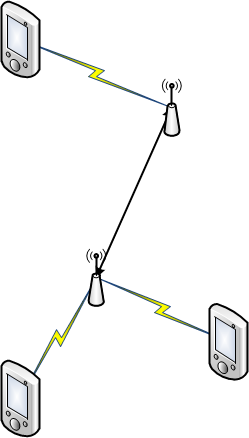
\includegraphics[width=0.3\textwidth]{images/background_net_infrastucture.png} }
	\hspace{15mm}
	\subfloat[Ad Hoc Mode]{\label{fig:adhoc_mode}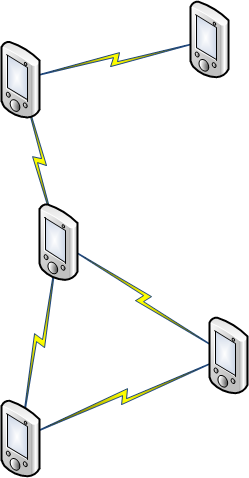
\includegraphics[width=0.3\textwidth]{images/background_net_adhoc.png}} 
	\caption{Difference between a regular infrastructure network and an ad hoc network}
	\label{fig:background_networks}
\end{figure}

Figure \ref{fig:background_networks} depicts the difference between regular
networks and ad hoc networks. In \ref{fig:infrastructure_mode} there are three
mobile nodes connected to each other through two wireless access points
(infrastructure), while in \ref{fig:adhoc_mode} there are five nodes connected
to each other and through each other. In infrastructure mode an end node only
accepts packets packets addressed to itself, while in ad hoc mode the node will
try to forward packets addressed to other nodes (on the network layer). They
will however not accept packets sent to other link-layer addresses.

A \ac{MANET} is a subset of ad hoc networks, in which nodes are specified as
non-stationary wireless nodes, i.e. a \ac{MANET} consists of several mobile
nodes communicating with each other, and through each other even while on the
move. With \acp{MANET} nodes are always on the move and must therefore update
their routing tables continously to make sure full paths between nodes are
updated as quickly as possible, i.e. a minimal routing path convergence is
necessary.

In this thesis the terms ``network'', ``\ac{MANET}'', and ``ad hoc network''
are used interchangeably meaning a ``\ac{MANET}'' as described in this section
unless otherwise specified.

\subsection{Routing}
There are many routing protocols for ad hoc networks and some of the popular
protocols are OLSR \cite{olsr_paper}, B.A.T.M.A.N. \cite{batman_rfc}, Babel
\cite{rfc6126}, DSDV \cite{he2002destination}, and AODV
\cite{Perkins:2003:AHO:RFC3561} which all fall into one of the two main
categories of ad hoc routing - i.e. ``reactive'' and ``pro-active'' routing
protocols.

\subsubsection*{Reactive Routing Protocols}


\subsubsection*{Pro-active Routing Protocols}


\subsection{Challenges}

\subsection{Security}

\section{B.A.T.M.A.N.}
BATMAN \cite{batman_rfc} is an increasingly more popular routing protocol for
wireless ad hoc networks, as seen by the fact its taken into the Linux kernel
net tree (\url{http://www.open-mesh.org/wiki/open-mesh/2011-03-17-batman-adv-and-the-penguin}).
The name is an abbreviation for ``Better Approach To Mobile Ad hoc Networking''.
The motivation behind developing BATMAN was to replace the Optimized Link State
Routing Protocol (OLSR) \cite{why-starting-batman} because of the inherent
difficulties that protocol has.

\subsection{From OLSR to BATMAN}
OLSR is a pro-active routing protocol, which means that participating nodes
regularly exchange routing information with each other. According to the BATMAN
developers the problem with OLSR is that every node in the network calculates
the whole routing path, which is a complex way to do it. Not only is it
difficult to make sure all nodes have the same information at the same time,
it also needs (relatively) much storage and computation time. If nodes sit on
different routing information this concept leads to routing loops and heavy
route flapping. The result is many patches to the protocol that defies the
protocol standard in order to make it more suitable \cite{why-starting-batman}.

The BATMAN developers therefore wanted to start with a clean slate. They decided
amongst other things that each node should only know the next hop, i.e. the
link-local neighbor that is the path between itself and the destination. In
many ways, what they did was to make a simpler and easier to understand
protocol. For instance, the way BATMAN calculates the optimal route, i.e. the
next jump, is by comparing the number of routing messages it has received from
each node and who was the last sender.

\subsection{BATMAN Protocol Explanation}
The routing messages sent in BATMAN are called \acp{OGM}. Figure
\ref{fig:original_ogm} show the packet format with all header fields. The
\ac{OGM} format has changed since the \cite{batman_rfc} was published, but there
is no official publication with the new packet format as of yet. The updated
packet format can be found in the project's internal documentation
\url{http://gitorious.org/batman-adv-doc/}. The packet format found in the RFC
belong to the older version III of the BATMAN algorithm. The algorithm used in
this thesis is version IV.

\begin{figure}[h]
	\centering
  	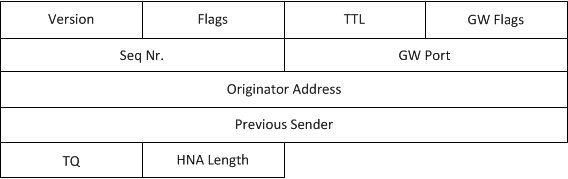
\includegraphics[width=\textwidth]{images/original_ogm.png}
  	\caption{BATMAN's \acf{OGM} packet format.}
	\label{fig:original_ogm}
\end{figure}

The real workhorse of the packet is the ``Originator Address'' field which
carries a host address of the node 'A' that broadcasted the \ac{OGM}. When a
node 'B' receives this message it checks if the originator address and source
address of the IP header are the same - if so the two nodes are direct
neighbors. B then forwards the \ac{OGM} only changing the ``\ac{TTL}'' and
``Previous Sender'' fields. All \acp{OGM} inside the BATMAN network are
broadcasted and rebroadcasted until the TTL has dropped to zero, or until they
receive an \ac{OGM} they have previously sent themselves.

This way all \acp{OGM} will be received and rebroadcasted by all nodes in the
network and all nodes will learn the existence of each other and which nodes are
the first hop between them and the other nodes, i.e. the first leg of the path.
All nodes and their first hops in their paths are stored in a list called an
``Originator List''.

\begin{figure}[h]
	\centering
	\subfloat{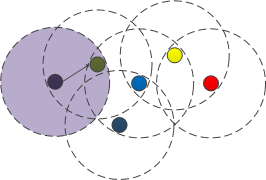
\includegraphics[width=0.3\textwidth]{images/ogm_packet_flow_1.png} }
	\subfloat{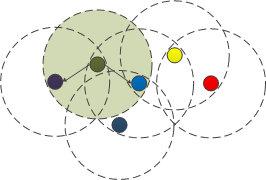
\includegraphics[width=0.3\textwidth]{images/ogm_packet_flow_2.png} } 
	\subfloat{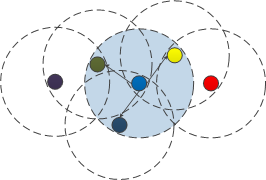
\includegraphics[width=0.3\textwidth]{images/ogm_packet_flow_3.png}}
	\\
	\subfloat{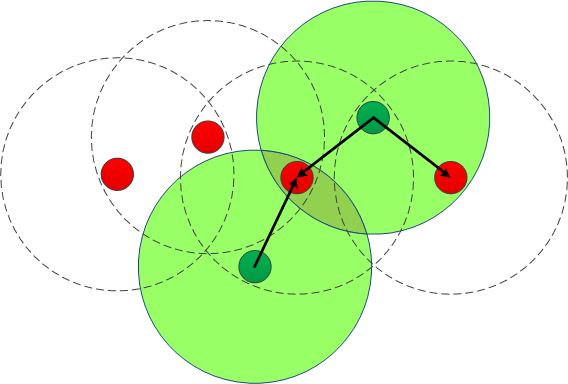
\includegraphics[width=0.3\textwidth]{images/ogm_packet_flow_4.png} } 
	\subfloat{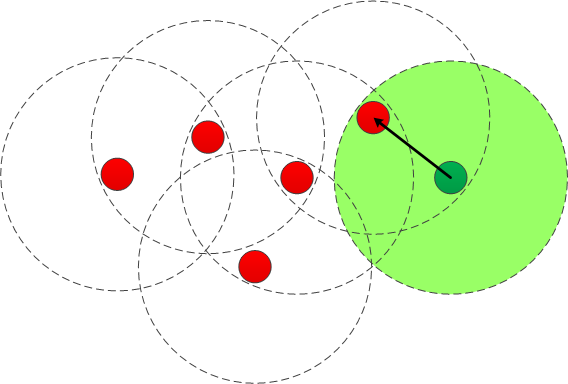
\includegraphics[width=0.3\textwidth]{images/ogm_packet_flow_5.png}}
	\caption{Flow of an \acf{OGM} originating from the left-most node.}
	\label{fig:ogm_packet_flow}
\end{figure}

Figure \ref{fig:ogm_packet_flow} shows how an \ac{OGM} is broadcasted and
forwarded through the network. The packet originates from the left-most node,
and for each node that receives the packet, they forward it to their neighbors
again.

When a node which has already received and forwarded an \ac{OGM} receives the
same \ac{OGM} from another node at a later point - it drops that packet so the
network will not get flooded by forwarding the same \acp{OGM} until its \ac{TTL}
is zero. This is also necessary in order to prevent routing loops.

\subsection{Batman Daemon vs. Batman-Advanced}

\section{Proxy Certificates}
\label{sect:pc}
A \acf{PC} is a X.509 Certificate ``(\ldots) derived from, and signed by, a
normal X.509 Public Key End Entity Certificate or by another Proxy Certificate
for the purpose of providing restricted proxying and delegation within a PKI
based authentication system.'' \cite{rfc3820}.

The idea behind \acp{PC} was to overcome challenges with authentication
using e.g. \ac{SSO} in a Grid Computing setting \cite{foster1998security}. Here
a user might want to initiate a process that runs over several entities in the
grid, and maybe even after the user has logged off. Therefore a way to delegate
the user's rights to the entities running the processes for him was necessary.

Simply understood, a \ac{PC} is a public key certificate signed not
by an \ac{CA}, but an \ac{EEC} or another \ac{PC}. With such certificates one
can delegate rights on behalf of one self, i.e. if you issue a \ac{PC} to some
other entity, that entity will be able to act on your behalf. \acp{PC} allows
the use of restrictions, given in a proxyPolicy field. This way the issuer can
decide which of its own rights the issuee will have, granted the issued \ac{PC}
cannot have more or elevated rights to that of the issuer of the \ac{PC}.

TODO: Mention entities PI, AC, AA\ldots Say something about why this can be
useful for our implementation. Maybe a figure with the certificate fields??


%PI - Proxy Issuer
%AC - Attribute Certificate
%AA - Attribute Authority

%Requirement from the RFC page 9: passing the PC request from entity B to
% entity A over an authenticated, integrity checked channel. In our solution
% this is OK because the out-of-band channel (fingerprint exchange) can be
% viewed as this authenticated integrity checked channel. . . me thinks

\section{Attacks on Mobile Ad Hoc Networks}
\subsection{Wormhole Attack}
\subsection{Blackhole Attack}
\subsection{Greyhole Attack}

\section{Related Work}

\subsection{A Secure Mobile Ad hoc Network Based on Distributed Certificate
Authority}
\cite{hosseinisecure} propose a solution for a secure MANET based on distributed
CA. They employ use of clusters and an offline/out-of-band authentication
scheme. They use RSA for encryption, because they claim it is more energy
efficient. READ AGAIN LATER\ldots

\subsection{A Threshold Cryptography Based Authentication Scheme for Mobile
Ad-hoc Network}
\cite{springerlink:Haimabati} have a more mathematical approach
to the problem. Requires predefined unique ID and special hardware with a hidden
and secure algorithm (i.e. smart card). This solution is probably better suited
for the military\ldots
